\subsection{Device under Test}
\label{sec::experiment}
\todo[inline]{Replace this section with Berdina}
Though experiments and designs are constantly evolving, at the core of this group's research is an \gls{set} used to perform electron spin readout. The apparatus I am applying my work to is by no means comprehensive, but it serves as a reference point in a proven device \cite{morello2010single}. To improve spin initialisation with this particular device would therefore be extensible to other devices and experiments.
Figure \ref{fig::thesis_experiment} shows a general layout used to control and read from an \gls{set}.

\begin{figure}[htbp!]
	\centering
	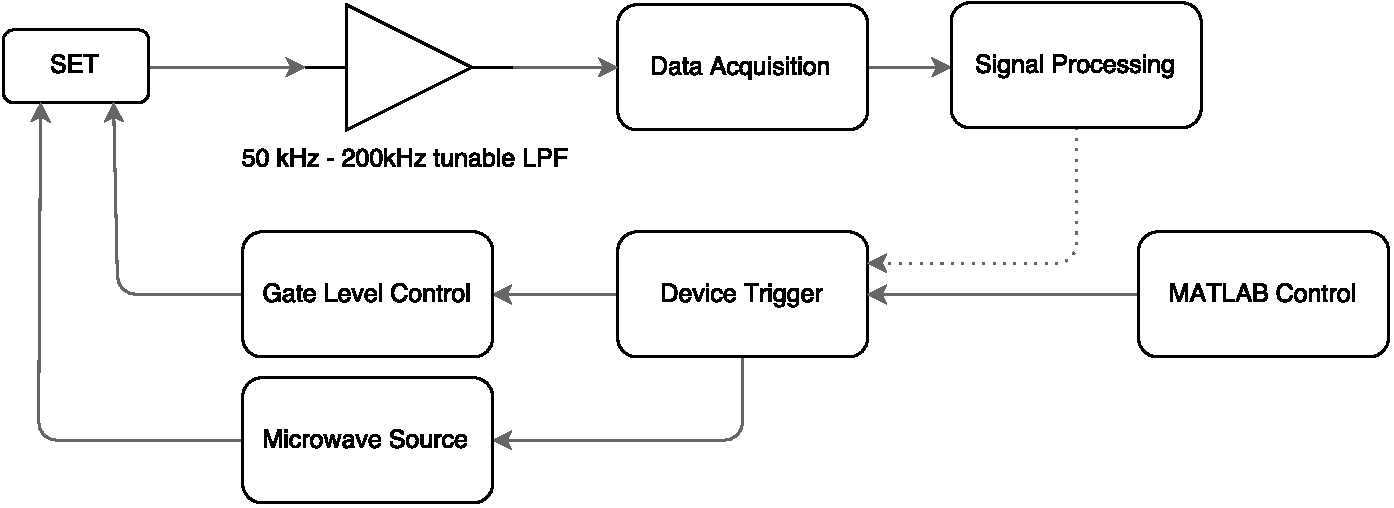
\includegraphics[width=\textwidth]{thesis_experiment.pdf}
	\caption{Block diagram of experiment}
	\label{fig::thesis_experiment}
\end{figure}


Figure \ref{fig::set_layout} shows the physical device that will be similar to one I will be testing my solution on. This devices has various voltage-controlled nodes, such as the top gate to induce a layer of electrons on the boundary, the left and right barriers to remove this layer, forming tunnel junctions to the island, and finally the plunger which can act at the gate as defined in section \ref{sec::set}.

\begin{figure}[htbp!]
	\centering
	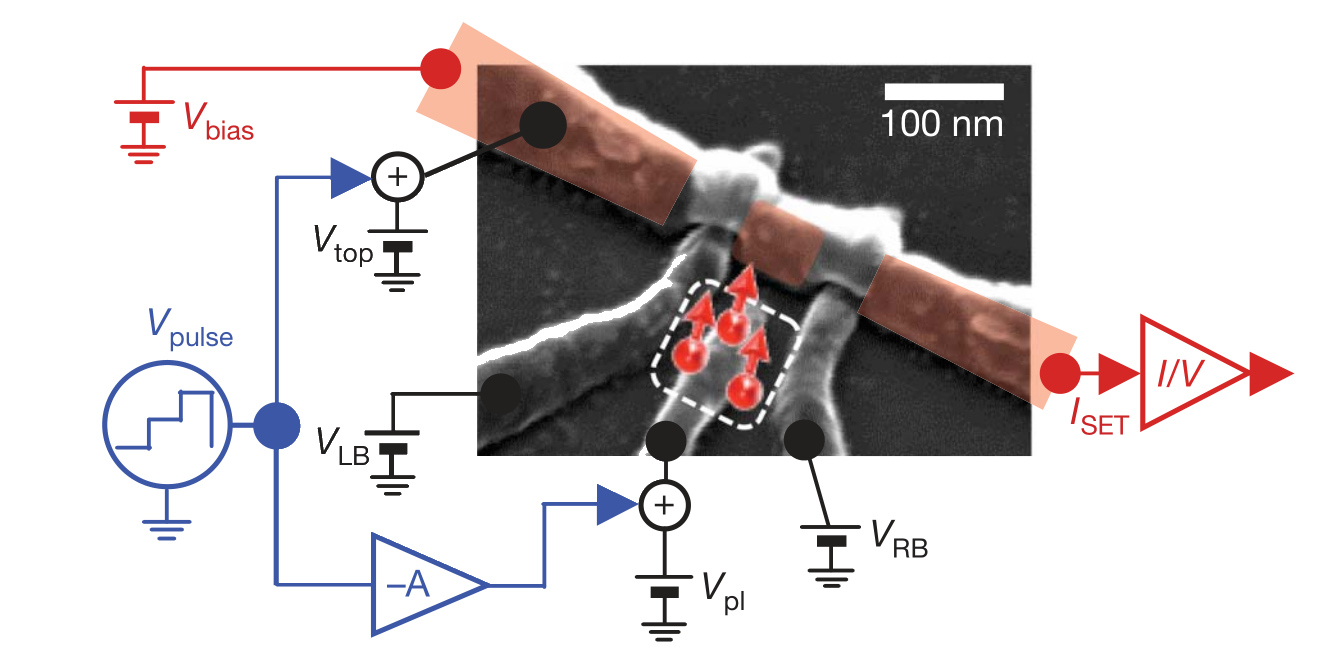
\includegraphics[width=\textwidth]{set_layout}
	\caption[Layout of an \gls{set}]{The layout of an \gls{set}\cite{morello2010single}}
	\label{fig::set_layout}
\end{figure}

\subsection{Problem Statement}
The problem with this current approach is the cost of running these experiments if at the point of the plunge there was no electron on the donor. Any data with an incorrect initialization must be discarded, so as not to disturb the results. To take this one step further, to require 99.9\% spin-down initialization fidelity would mean ignoring over 90\% of all recorded data. This kind of waste can be circumvented by a feedback loop that can decide when the initialization has been performed correctly, and thus continue the experiment.

The problem I am to solve in this thesis is to incorporate digital feedback with current research, closing the loop in Figure \ref{fig::thesis_experiment}, which will allow for experiments to run more efficiently and lessen the burden on the researchers in selecting their data. The following section will detail some available solutions.

\subsection{Process}

	\subsubsection{Electrostatic and Electrodynamic Stimulus}
	\todo[inline]{Add pulse sequence explanation here}
	To allow for precise control and measurement of the steering time applied to the electron donor, an electrostatic environment needed to be defined, along with radio and microwave stimulus. The SET donor is coupled capacitively to a number of gates.
	